\documentclass[a4paper, 12pt]{article}
\usepackage{geometry}
\geometry{margin=2cm}
\usepackage{graphicx} % Required for the inclusion of images
\usepackage[utf8]{inputenc}
%\usepackage{natbib} % Required to change bibliography style to APA
\usepackage{amsmath} % Required for some math elements 
\usepackage[spanish]{babel} 
%\usepackage{fontspec}
\usepackage{lineno,hyperref}
\usepackage{upgreek}
\usepackage{gensymb}
\usepackage{textcomp}
\usepackage{amssymb}
\usepackage{textgreek}
\usepackage{float}
\usepackage{fancyhdr}
\usepackage{dirtytalk}

\allowdisplaybreaks
%\textwidth18cm
%\textheight22cm
%\topmargin0cm
%\oddsidemargin2cm
%\hypersetup{hidelinks}

\usepackage{multirow}

\hypersetup{
    colorlinks=true,
    linkcolor=blue,
    }
\graphicspath{{img}}
\setlength\parindent{0pt} % Removes all indentation from paragraphs

\renewcommand{\labelenumi}{\alph{enumi}.} % Make numbering in the enumerate environment by letter rather than number (e.g. section 6)

\renewcommand{\b}{\bf}

\newsavebox{\mygraphic}
\sbox{\mygraphic}{
\includegraphics[height=1cm]{logoUNRN.jpg}}


\pagestyle{fancy}

\fancyhead{}

\headheight 16pt

\fancyhead[LO]{\setlength{\unitlength}{1in}
	\begin{picture}(0,0)
		\put(0,0){\usebox{\mygraphic}}
	\end{picture}
	\hspace{1cm}
}

\fancyhead[CO] {\hspace{1.5cm} \large Física I: Ingenierías Ambiental, Electrónica y Telecomunicaciones}

%esto me pareció piola para enumerar los ejercicios
%lo saqué de acá: https://tex.stackexchange.com/questions/302948/numbered-exercises-as-sections
%%%%%%%%%%%%%%%%%%%%%%%%%%%%%%%%%%%%%%%%%5
\newcounter{eje}
\setcounter{eje}{0}
\newcounter{subeje}
\setcounter{subeje}{-1}
\renewcommand\thesubeje{\arabic{eje}\alph{subeje}}%
\newcommand \eje{%
  \vspace{.2cm}
  \par\noindent
  \ifnum\value{subeje}>-1
    \refstepcounter{subeje}%
    \llap{\thesubeje)\quad}%
  \else
    \refstepcounter{eje}%
    \llap{\theeje)\quad}%
  \fi
}
\begin{document}
\pagestyle{fancy}

\begin{center}

	{\Large \bf{Final Física I (Diciembre 2023)}}
 
\vspace{.2cm}

{miércoles 20/12}
\end{center}

%\hspace{5cm}Tome para el valor de g = 9.8 m/s$^2$.
\begin{itemize}
	\item Resuelva cada ejercicio en una hoja separada
	\item Si las cantidades que se piden son dimensionales, acompañe el valor con la unidad correspondiente
	\item De las respuestas con precisión numérica consecuente con los datos
	\item para la gravedad utilice g = 9.8 m/s$^2$.
\end{itemize}

\eje {\bf [muy parecido a ejercicios nuevos práctica 1]} Un piloto desea que su aeronave vuele en dirección norte respecto del suelo, pero hay viento de 60.0 km/hr que sopla de oeste a este (izquierda a derecha).
\begin{itemize}
\item [a)] Si la velocidad del avión con respecto al viento es de 320.0 km/hr, ¿hacia dónde debe dirigir la aeronave, el piloto, para lograr ir hacia el norte?

\item [b)] ¿Cuál es la velocidad del avión respecto del suelo?

\item [c)] Muestre en un gráfico los vectores velocidad involucrados en la resolución del problema.
\end{itemize}

\eje {\bf [nuevo]} El bloque con forma de cuña de la figura adjunta se acelera de tal manera que el carrito sobre este, no desliza por la pendiente, es decir que no lo hace ni para arriba, ni para abajo. Despreciando el rozamiento entre el carrito y el bloque, encuentre la aceleración de la cuña para que esto ocurra

\begin{figure}[H]
\begin{center}
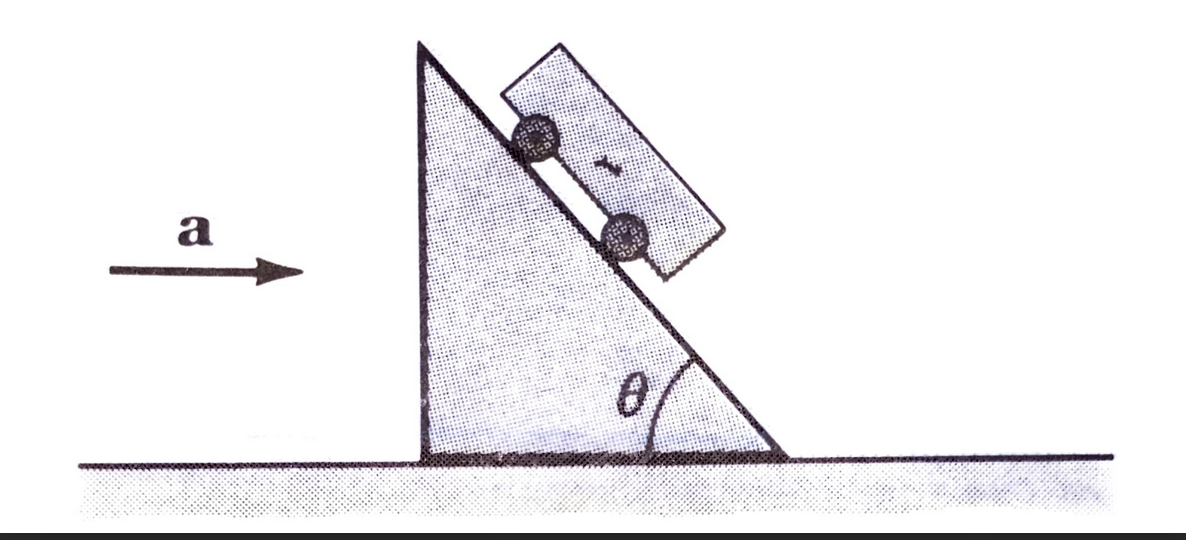
\includegraphics[clip,width = .45\columnwidth]{img/integrador2023-0.png}
\end{center}
\end{figure}

\eje {\bf [eje 16 práctica 5 hecho por Raúl]} Un cilindro sube por el plano inclinado por la acción de un par de fuerzas (es decir, fuerzas iguales y opuestas) que generan un torque M, como indica la figura. 
\begin{itemize}
\item [a)] Realizar el diagrama de cuerpo libre del cilindro COMPLETO. Todas las fuerzas y todos los torques (respecto del CM).

\item [b)] Hallar el valor máximo que puede tener el par de fuerzas aplicado para que el cilindro suba por el plano rodando sin deslizar. 

\item [c)] Hallar la aceleración del centro de masa del cilindro para que éste suba por el plano rodando sin deslizar 
\end{itemize}

\begin{figure}[H]
\begin{center}
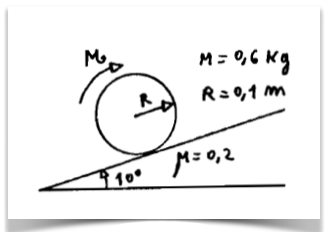
\includegraphics[clip,width = .35\columnwidth]{img/2doparcial2023-0.png}
\end{center}
\end{figure}

\eje {\bf [nuevo]} Un carrito de masa M = $0.25$ kg, inicialmente en reposo, se deja caer por un plano inclinado para luego tomar una rampa que lo deja en caída libre al ras del suelo, forzando una dirección de 30$\degree$ en la velocidad inicial. Luego del vuelo libre el carrito vuelve a tocar el suelo a una distancia $d = 1$m., Si el carrito se soltó desde una altura $h = 1.5$m
\begin{itemize}
  \item[a)] Determine el trabajo de las fuerzas no conservativas (sin omitir el signo ya sea positivo o negativo)
  %rta Wnc = Ef - Ei = K - Upot = 1/2 M g d/sen(60) - Mgh = -0.35m Mg = -0.846 J
  
  \item[b)] Suponiendo que las fuerzas no conservativas actúan únicamente a lo largo de 2 metros del plano inclinado, ¿cuál será el coeficiente de roce dinámico $\mu_d$? Realice un diagrama de cuerpo libre si fuera necesario.
% rta: Wnc = -1* Mgcos(37) * \mu * 2 m = -0.35 Mg  --> \mu =0.35/2/0.8 = .22
  
  \item[c)] ¿Qué fracción de la energía potencial inicial se disipa por el trabajo de las fuerzas de roce? (Considere el cero a nivel del suelo)
  
%  rta:   Upot * q = |Wnc|
%         Mg 1.5m q = 0.35m Mg --> q = 0.23

  \item[d] ¿Cuál es el módulo de la velocidad al inicio del vuelo libre?  
  %acá está la clave del problema
  %rta v0 = \sqrt{g d /sen(2\theta)} = 3.37 m/s
\end{itemize}
\begin{figure}[H]
\begin{center}
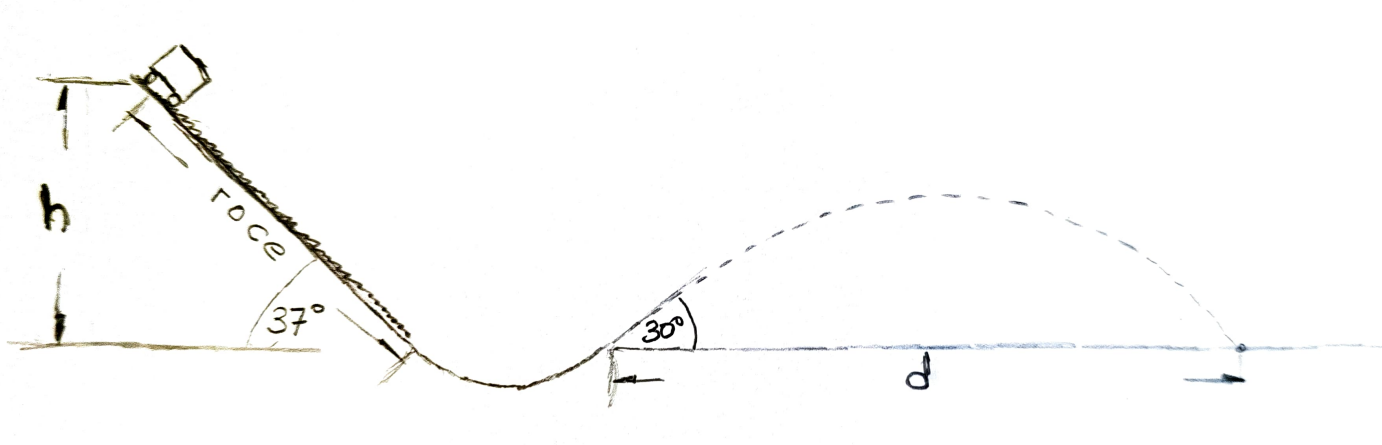
\includegraphics[clip,width = \columnwidth]{img/ener-roce_final_dic2023.png}
\end{center}
\end{figure}

\eje {\bf [tomado de 2do parcial 2023]} Una plataforma realiza un MAS según una dirección vertical con amplitud A = 0.5 m. 

a) ¿Cuál debe ser el período mínimo de oscilación para que un cuerpo colocado sobre la plataforma no se separe de ella? 

b) Luego, ¿qué pasaría si el período fuera aún menor?

\eje {\bf [eje 8 práctica 10 hecho por Raúl]} En una transformación a presión constante (presión atmosférica) el volumen de un gas varía en 0.25 litros. Se le suministran 21.8 cal. En una transformación a volumen constante se le suministran 15.6 cal. Calcular en ambos casos la variación de la energía interna del gas.
\end{document}